\section{Deep-Q-Learning Experimente}
\subsection{Das Prinzip von Deep-Q-Learning} \label{sec:deepQPrinciple}
Bisher haben wir alle Q-Values in einer Q-table gespeichert. Dieses Vorgehen ist relativ simpel, stößt aber nach \cite{11_maxim2018deeprl} bei großen Zustands- bzw. Aktionsräume schnell an seine Grenzen. Als Beispiel wird hier Q-Learning bei Atari-Spielen aufgeführt, bei denen die Pixel als Zustände benutzt werden. Es leuchtet ein, dass in so einem Fall aufgrund der großen Menge an state-action Paaren die Speicherung deren Q-values schwierig, wenn nicht sogar unmöglich ist.

Nach \cite{11_maxim2018deeprl} ist die Benutzung von Neuronalen Netzen eine der populärsten Methoden, um mit diesem Problem umzugehen. Wir kombinieren Q-Learning mit einem Neuronalen Netz und erhalten auf diese Weise ein so genanntes \textit{Deep-Q-Network} (\textit{DQN}).

Für das stabile und effiziente Trainieren eines DQNs gibt es nach \cite{11_maxim2018deeprl} einige Techniken und Tricks. Die Informationen diesbezüglich wurden -- falls nicht anders angegeben -- aus \cite{11_maxim2018deeprl} entnommen.

\paragraph{$ \epsilon $-greedy}
Die $ \epsilon $-greedy Strategie löst das Exploration versus Exploitation Dilemma. Da wir uns hiermit bereits in Kapitel \ref{sec:exploration_exploitation} befasst haben, halten wir uns an dieser Stelle nicht weiter damit auf.

\paragraph{Replay buffer}
Die Daten, die der Agent im Laufe des Trainings sammelt, sind nicht unabhängig voneinander. Sie liegen höchst wahrscheinlich sehr nahe beieinander, da sie meist zur selben Episode gehören. Dazu kommt, dass die Verteilung der Daten durch die aktuelle Policy, beziehungsweise bei der Verwendung von $ \epsilon $-greedy teilweise zufällig bestimmt wird. Wünschenswert wäre eine Verteilung der Trainingsdaten identisch zu Stichproben unter Verwendung der optimalen Policy, die wir erlernen wollen.

Um dem entgegenzuwirken verwenden wir einen großen Speicher, welcher unsere vergangenen Beobachtungen enthält. Anstatt nun mit den letzten Beobachtungen zu trainieren, entnehmen wir zufällig Daten aus diesem Speicher. Diese Methode nennt man \textit{replay buffer}. In Kapitel \ref{sec:qLearningImplementation} verwenden wir ebenfalls einen solchen replay buffer.

\paragraph{Target network}
Ein ähnliches Problem stellt der Zusammenhang zwischen benachbarten Schritten dar. Die Bellman equastion aus \ref{eq:bellman} besagt, dass wir den Wert von $ q_\pi(s, a) $ über $ q_\pi(s', a') $ berechnen können. Die Zustände $ s $ und $ s' $ sind allerdings nur einen Schritt voneinander entfernt. Sie sind also sehr ähnlich und vom Neuronalen Netz schwer zu unterscheiden. Das hat zur Folge, dass wir bei einem Update der Parameter des Netzes für die Annäherung von $ q_\pi(s, a) $ an das gewünschte Resultat indirekt auch den Wert für $ q_\pi(s', a') $ verändern können. Dies kann das Training sehr instabil machen.

Deshalb verwenden wir ein so genanntes \textit{target network}. Das target network ist eine Kopie des training networks -- bei uns später auch policy network genannt --, welches lediglich alle $ N $ Schritte oder Episoden synchronisiert wird. $ N $ ist hierbei ein weiterer Hyperparameter, den wir bei später als \mintinline{python}{target_update} bezeichnen. Mit dieser Kopie besitzen wir nun fixierte Werte für $ q_\pi(s', a') $, was das Training wesenlicht stabiler machen sollte.

\paragraph{Der Trainingsablauf von DQN}
Wir betrachten nun einen klassischen Algorithmus für DQN. \cite{11_maxim2018deeprl} entnimmt dessen Schritte den bekannten Papern \textit{Playing Atari with Deep Reinforcement Learning} \cite{13_mnih2013atari} und \textit{Human-Level Control Through Deep Reinforcement Learning} \cite{12_mnih2015humanlevel}. Sinngemäß wiedergegeben ist der Ablauf nach \cite{12_mnih2015humanlevel} wiefolgt:
\begin{enumerate}[nosep]
    \item Initialisieren der replay memory Kapazität
    \item Initialisieren des Hauptnetzes mit zufälligen Parametern
    \item Kopie des Hauptnetzes anlegen, das target network
    \item \textit{For each Episode do}
    \begin{enumerate}
        \item Startzustand initialisieren
        \item \textit{For each Zeitschritt do}
        \begin{enumerate}
            \item Auswahl einer Aktion via $ \epsilon $-greedy
            \item Ausführen der Aktion in einem Emulator
            \item Beobachten der Belohnung und des Folgezustands
            \item Speichern der Beobachtung im replay memory
            \item Zufällige Auswahl einer Reihe von Beobachtungen (batch) aus dem replay memory
            \item Vorverarbeitung der Zustände
            \item loss (TODO) zwischen Q-values und Ziel-Q-values berechnen (Benutzung des target networks für den Folgezustand)
            \item Aktualisieren der Gewichte im Netz, um den loss zu minimieren
            \item Alle $ N $ Episoden wird das target network mit dem Hauptnetz synchronisiert
        \end{enumerate}
    \end{enumerate}
\end{enumerate}
In unserem Fall kommt noch ein weiterer Schritt hinzu, in dem wir das aktuelle Netz kopieren und als \mintinline{python}{best_net} speichern, wenn der moving average einen neuen Höchstwert erreicht. Dieses Netz wird dann am Ende des Trainings zurückgegeben. Dies soll sicherstellen, dass zum Schluss das beste Trainingsergebnis ausgegeben wird, auch wenn der Agent im Laufe der Zeit Sachen wieder verlernt hat. Wir ergänzen also:
\begin{enumerate}
    \item[4.] \textit{(Fortsetzung)} 
    \begin{enumerate}
        \item[c)] Bei neuer Höchstleistung des Trainings Synchronisation des Ausgabenetzes mit dem Hauptnetzes
    \end{enumerate}
\end{enumerate}

\subsection{Implementierung in Python}
Wir wollen nun einen DQN-Agenten in Python implementieren. PyTorch ist eine beliebtes Deep-Learning-Framework, welches Benutzerfreundlichkeit und Leistung vereint \cite{x01_pytorch}. Als Grundlage verwenden wir das Codebeispiel unter \url{https://github.com/philtabor/Youtube-Code-Repository/blob/master/ReinforcementLearning/DeepQLearning/torch_deep_q_model.py} (Zugriff am 30.03.2021), welches für unsere Zwecke stark modifiziert wird. Das Zentrum des Geschehens ist wieder die \mintinline{python}{train()}-Methode. Der besseren Übersicht wegen sind hier einige weniger relevante Codeausschnitte herausgekürzt (gekennzeichnet mit ...). Außerdem wurde die Einrückung auf der Ebene der Methode entfernt. Die Schritte sind entsprechend der Liste aus \ref{sec:deepQPrinciple} nummeriert:
\begin{minted}[texcomments]{python}
def train(width: int, length: int, params, environment, ... ):
agent = Agent( ... ) # 1. bis 3.
scores, eps_history = [], []
max_average = -99999
for episode in range(params.num_episodes): # 4.
    score = 0
    environment.reset_agent() # a)
    observation = environment.get_state_for_deep_q(step=0, ... ) # a)
    for step in range(params.max_steps_per_episode): # b)
        action = agent.choose_action(observation) # i.
        state, reward, done = environment.agent_perform_action(
            action, ... )
        ) # ii. und iii.
        observation_ = environment.get_state_for_deep_q(step=step, ...)
        # iii.
        score += reward
        agent.store_transition(
            observation, action, reward, observation_, done
        ) # iv.

        agent.learn(episode) # v. bis ix.)

        observation = observation_
        # ... falls gewünscht Position des Agenten anzeigen
    # ... falls gewünscht Pfad des Agenten anzeigen
    scores.append(score)
    agent.exploration_rate = params.min_exploration_rate +\
        (params.max_exploration_rate - params.min_exploration_rate) *\
        np.exp(-params.exploration_decay_rate * episode)
    # ... falls gewünscht Trainingsfortschritt als Graph ausgeben
    current_average = get_current_average( ... )
    if max_average < current_average or episode == plot_moving_avg_period:
        max_average = current_average
        agent.best_net.load_state_dict(agent.policy_net.state_dict())# c)
params.rewards_all_episodes = scores
params.max_reward_average = max_average
return agent.best_net, params
\end{minted}
Die Schritte 1. bis 3. passieren bei der Initialisierung des Agenten und sind relativ unspektakulär. Interessanter ist die \mintinline{python}{learn()}-Methode des Agenten, die in jedem Zeitschritt einmal aufgerufen wird und die Schritte v. bis ix. abdeckt. Wir werfen daher einen blick auf deren Code. Auch hier wurde aus Platzgründen die Einrückung auf der Ebene der Methode entfernt:
\begin{minted}{python}
def learn(self, episode):
if self.memory_counter < self.batch_size:
    return # return, falls noch nicht genügend Beobachtungen existieren
self.policy_net.optimizer.zero_grad()

max_mem = min(self.memory_counter, self.mem_size)
batch = np.random.choice(max_mem, self.batch_size, replace=False) # v.

batch_index = np.arange(self.batch_size, dtype=np.int32)
state_batch =\
    T.tensor(self.state_memory[batch]).to(self.policy_net.device)
new_state_batch =\
    T.tensor(self.new_state_memory[batch]).to(self.policy_net.device)
reward_batch =\
    T.tensor(self.reward_memory[batch]).to(self.policy_net.device)
terminal_batch =\
    T.tensor(self.terminal_memory[batch]).to(self.policy_net.device)
action_batch = self.action_memory[batch]
 # vii. Start
q_eval = self.policy_net.forward(state_batch)[batch_index, action_batch]
q_next = self.target_net.forward(new_state_batch)
q_next[terminal_batch] = 0.0
q_target = reward_batch + self.gamma * T.max(q_next, dim=1)[0]
loss = self.policy_net.loss(q_target, q_eval).to(self.policy_net.device)
loss.backward()
 # vii. Ende
self.policy_net.optimizer.step() # viii.

if episode % self.target_update == 0:
    self.target_net.load_state_dict(self.policy_net.state_dict()) # ix.
\end{minted}
Zuletzt betrachten wir noch die Klasse \mintinline{python}{DeepQNetwork}, welche das DQN modelliert:
\begin{minted}{python}
class DeepQNetwork(BasicNetwork):
    def __init__(self, learning_rate, input_dims, fc1_dims, fc2_dims,
                 n_actions):
        super(DeepQNetwork, self).__init__()
        self.learning_rate = learning_rate
        self.input_dims = input_dims
        self.fc1_dims = fc1_dims
        self.fc2_dims = fc2_dims
        self.n_actions = n_actions

        self.fc1 = nn.Linear(*self.input_dims, self.fc1_dims)
        self.fc2 = nn.Linear(self.fc1_dims, self.fc2_dims)
        self.out = nn.Linear(self.fc2_dims, self.n_actions)
        self.optimizer = optim.Adam(self.parameters(),
                                    lr=learning_rate)
        self.loss = nn.MSELoss()
        self.device =\
            T.device('cuda' if T.cuda.is_available() else 'cpu')
        self.to(self.device)

    def forward(self, state):
        x = T.sigmoid(self.fc1(state))
        x = T.sigmoid(self.fc2(x))
        actions = self.out(x)
        return actions
\end{minted}
Wir verwenden in unserem DQN zwei sogenannte Fully-connected hidden Layers. Das bedeutet, dass alle Neuronen einer Schicht mit allen Neuronen der nächsten Schicht verknüpft sind. PyTorch nutzt hierfür die Bezeichnung \mintinline{python}{Linear} layer. Die erste Ebene nimmt Eingaben mit den Dimensionen \mintinline{python}{input_dims} entgegen. Wir legen die Dimensionen der beiden hidden Layers für die folgenden Experimente auf \mintinline{python}{fc1_dims = 256} und \mintinline{python}{fc2_dims = 256} fest. Die Anzahl an Outputs der Ausgabeebene entspricht der Anzahl der Aktionen, die dem Agenten zur Verfügung stehen. In unserem Fall sind das \mintinline{python}{n_actions = 4}, also die vier möglichen Bewegungsrichtungen oben, rechts, unten und links.

Die ReLU activation function wird im Moment als die mit der besten Performance angesehen \cite{10_stevens2020deep}. Trotzdem benutzen wir für unsere activation function Sigmoid, das diese in unserem Anwendungsfall bessere Ergebnisse zu erziehlen scheint (TODO belegen). 

Die Hyperparameter werden in der Datenklasse \mintinline{python}{DeepQParameters} verwaltet. Diese enthält die gleichen Parameter wie \mintinline{python}{Parameters} aus Kapitel \ref{sec:qLearningHyperparameter}, wird aber noch um folgende ergänzt:
\begin{minted}{python}
@dataclass
class DeepQParameters:
    # ... wie in Parameters
    replay_buffer_size: int
    batch_size: int
    target_update: int
\end{minted}
Deren Funktion wurde im Kapitel \ref{sec:deepQPrinciple} bereits erläutert.

\subsection{Erste Experimente} \label{sec:deepQFirstExperiments}
Wir wollen diese Implementierung nun für einige Experimente nutzen. Ziel ist es zunächst, eine geeignete Aufgabe für den Agenten zu finden, welche anschließend für den Vergleich unterschiedlicher Lernstrategien dienen soll.

\paragraph{TODO}
Das DQN erhält als Eingabe die aktuelle Position des Agenten in Form einer x- und einer y-Koordinate. Diese beschreiben in diesem Experiment den Zustand des Agenten. Die Mitte der Landschaft hat die Koordinaten (0, 0). Dies ist ebenfalls der Startpunkt des Agenten. Als Belohnung erhält der Agent wie in Kapitel \ref{sec:qLearningExperiments} die Differenz der Höhe des Folgezustands und des aktuellen Zustands. Die Hyperparameter werden wie folgt belegt:
\begin{minted}{python}
params = DeepQParameters(
            num_episodes=10000,
            max_steps_per_episode=100,
            replay_buffer_size=20000,
            batch_size=32,
            learning_rate=0.001,
            discount_rate=0.999,
            target_update=25,
            start_exploration_rate=1,
            max_exploration_rate=1,
            min_exploration_rate=0.001,
            exploration_decay_rate=0.001,
            # ... Rest wird erst während des Trainings belegt
        )
\end{minted}
Damit einzelne Beobachtungen nicht zu einer völligen Veränderung der Gewichte im DQN führen, ist die \mintinline{python}{learning_rate} im Vergleich zum Training mit der Q-table sehr klein.
\begin{figure}[H]
    \centering
    \begin{subfigure}[b]{0.49\textwidth}
        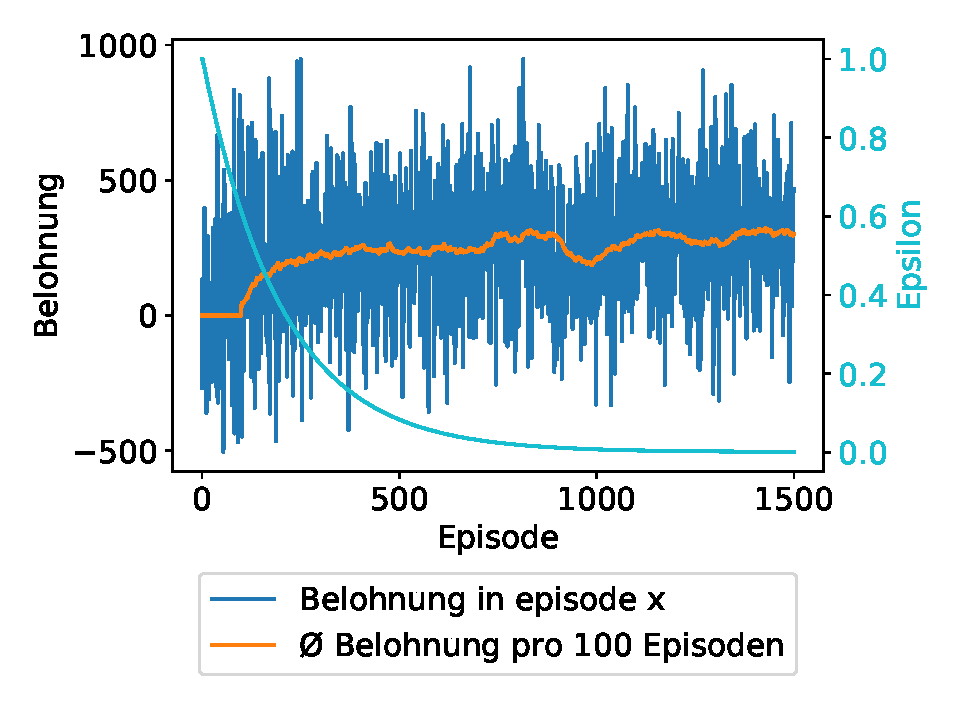
\includegraphics[width=\textwidth]{deep_q_learning/figure_simple.pdf}
        \caption{TODO}
        \label{img:graphDeepQSimple}
    \end{subfigure}
    \begin{subfigure}[b]{0.49\textwidth}
        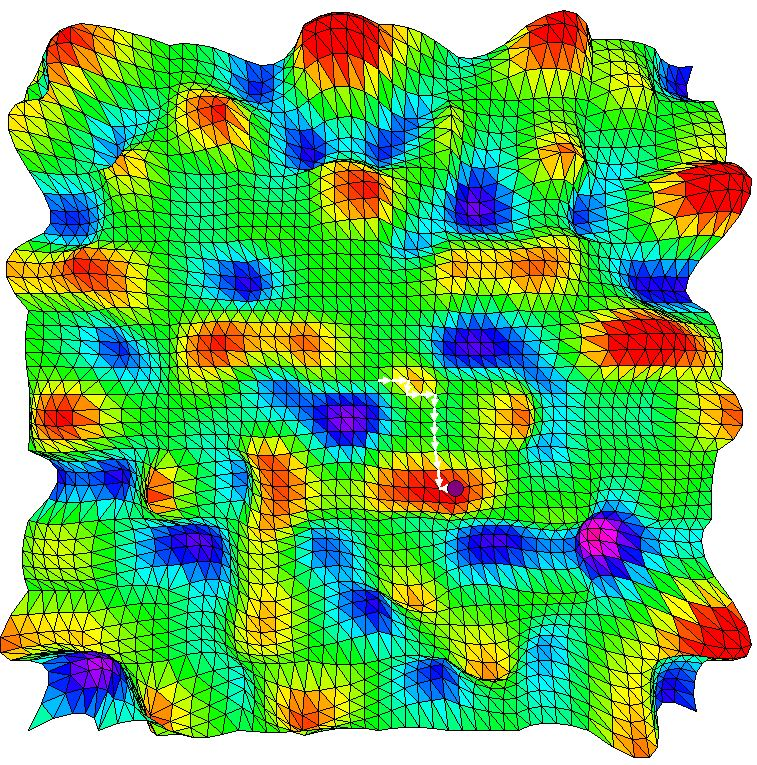
\includegraphics[width=\textwidth]{deep_q_learning/terrain_path_simple.JPG}
        \caption{TODO}
        \label{img:pathDeepQSimple}
    \end{subfigure}
    \caption{Ergebnisse des ersten Experiments}
\end{figure}
Der Agent scheint mit diesen Informationen noch nicht viel anfangen zu können. Der Graph \ref{img:graphDeepQSimple} zeigt, dass der moving average Wert (orange Linie) über die komplette Trainingszeit sehr Inkonsistent ist. Außerdem liegt er größtenteils deutlich unter dem möglichen Höchstwert. Dies lässt sich daran erkennen, dass die blaue Linie -- also die Belohnung der einzelnen Episoden -- teilweise fast bis 400 geht, der moving average diesen aber nur wenige Male fast erreicht. In Abbildung \ref{img:pathDeepQSimple} ist zu erkennen, welchen Pfad der Agent unter Verwendung des aus dem Training resultierenden Netzes zurücklegt. Er geht auf einen Gipfel, welcher sich Nahe am Startzustand befindet. Optimal wäre jedoch der Gipfel ganz oben in der Mitte.

Das DQN liefert hier also kein sonderlich gutes Ergebnis. Dies könnte daran liegen, dass der Agent keinerlei Information über die Höhe seiner Zustände hat, von denen seine erhaltene Belohnung und die Erfüllung der Aufgabe ja stark abhängt.

\paragraph{TODO}
 Wir passen also die Werte an, die einen Zustand beschreiben und fügen die Höhe des aktuellen Zustands, sowie die der umliegenden Zustände hinzu. Das DQN erhält also nun als Eingabe sieben Werte (x- und y-Koordinate, eigene Höhe und die Höhe der vier umliegenden Felder).

Das letzte Training hat für die 10000 Episoden auf einer Nvidia RTX 2060 (TODO evtl. unnötig zu erwähnen?) etwas über eineinhalb Stunden gedauert. Wir suchen eine Aufgabe, die für den Vergleich unterschiedlicher Lernstrategien genutzt werden soll und wollen für jede Strategie eine Experimentreihe durchlaufen, um eine statistische Auswertung zu ermöglichen. Diese sollten in zumutbarer Zeit durchführbar sein. Daher ist es wichtig, die Trainingszeit für einzelne Experimente zu reduzieren. 

Wir reduzieren daher die Episodenanzahl \mintinline{python}{num_episodes} auf 1500. Dementsprechend muss auch die \mintinline{python}{exploration_decay_rate} angepasst werden. Wir setzen diese auf 0.005.
\begin{figure}[H]
    \centering
    \begin{subfigure}[b]{0.49\textwidth}
        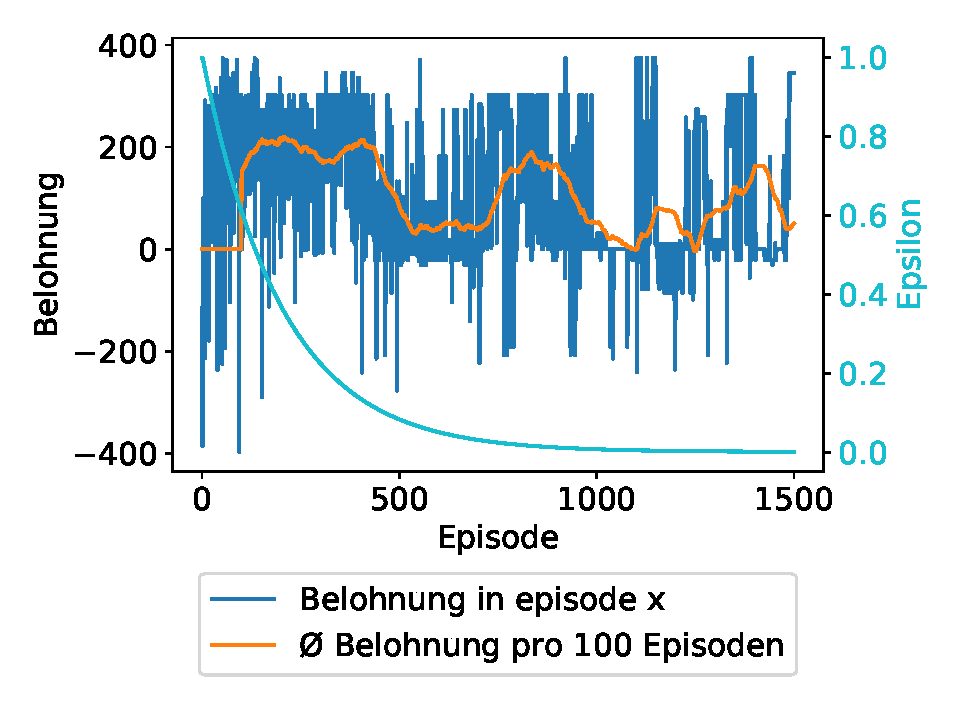
\includegraphics[width=\textwidth]{deep_q_learning/figure_height_in_state.pdf}
        \caption{TODO}
        \label{img:graphDeepQHeightInState}
    \end{subfigure}
    \begin{subfigure}[b]{0.49\textwidth}
        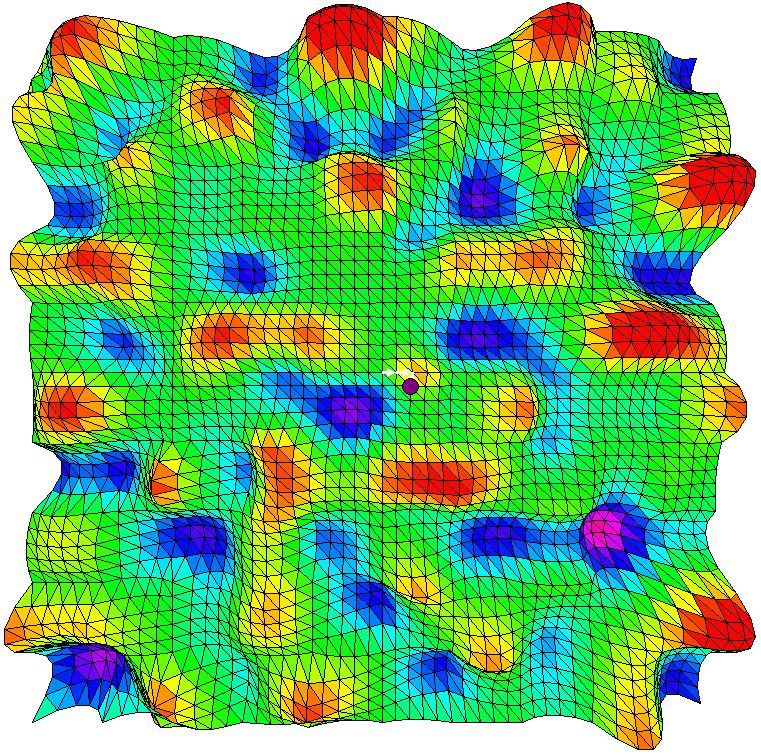
\includegraphics[width=\textwidth]{deep_q_learning/terrain_path_height_in_state.JPG}
        \caption{TODO}
        \label{img:pathDeepQHeightInState}
    \end{subfigure}
    \caption{Ergebnisse des ersten Experiments}
\end{figure}
In Abbildung \ref{img:pathDeepQHeightInState} lässt sich schnell erkennen, dass das Trainingsergebnis auch hier nicht zufriedenstellend ist. Der Agent bewegt sich nur ein paar Felder weit zu einem nahe gelegenen, sehr kleinen Hügel. Der moving average in Graph \ref{img:graphDeepQHeightInState} zeigt auch keinen gewünschten Trainingsverlauf wie beispielsweise in Graph \ref{img:graphQBest}. Lediglich die Trainingsdauer hat sich wie erwartet verringert.

\paragraph{Zufällige Startposition}
Wir werden daher unseren Ansatz etwas verändern. Die Startposition wird zu Beginn jeder Episode zufällig gewählt. Das DQN erhält außerdem statt der absoluten Position im Grid die relative Position zum Startpunkt. Das bedeutet, dass dieser immer die Koordinaten (0, 0) besitzt. Dies soll die Abhängigkeit von einem immer gleichen Startzustand aufbrechen und die Aufgabe interessanter machen.
\begin{figure}[H]
    \centering
    \begin{subfigure}[b]{0.49\textwidth}
        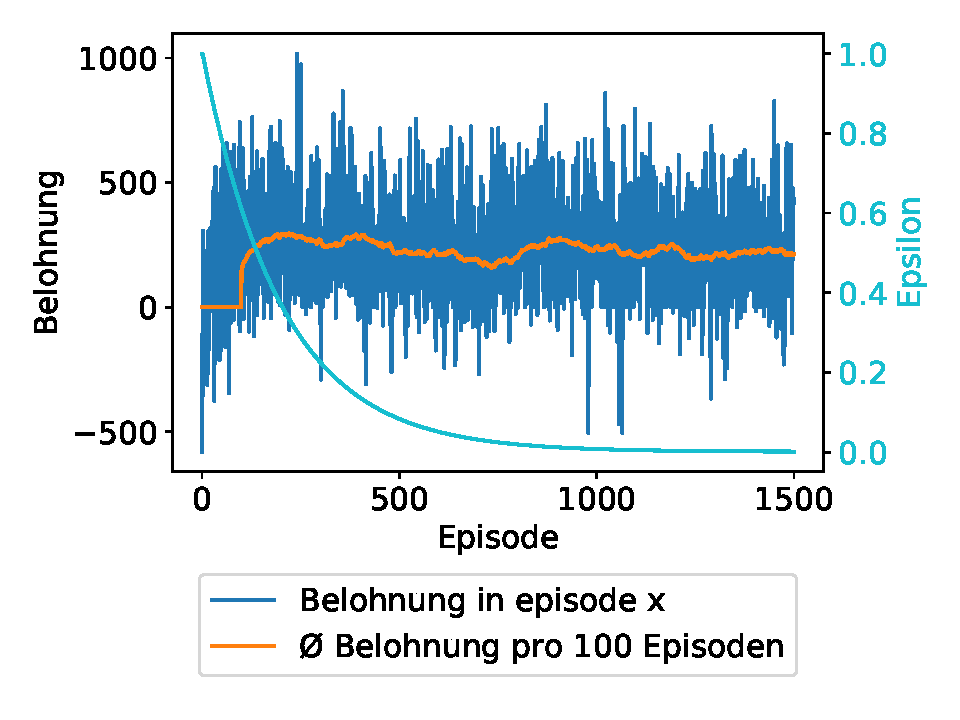
\includegraphics[width=\textwidth]{deep_q_learning/figure_random_spawn.pdf}
        \caption{TODO}
        \label{img:graphDeepQRandomSpawn}
    \end{subfigure}
    \begin{subfigure}[b]{0.49\textwidth}
        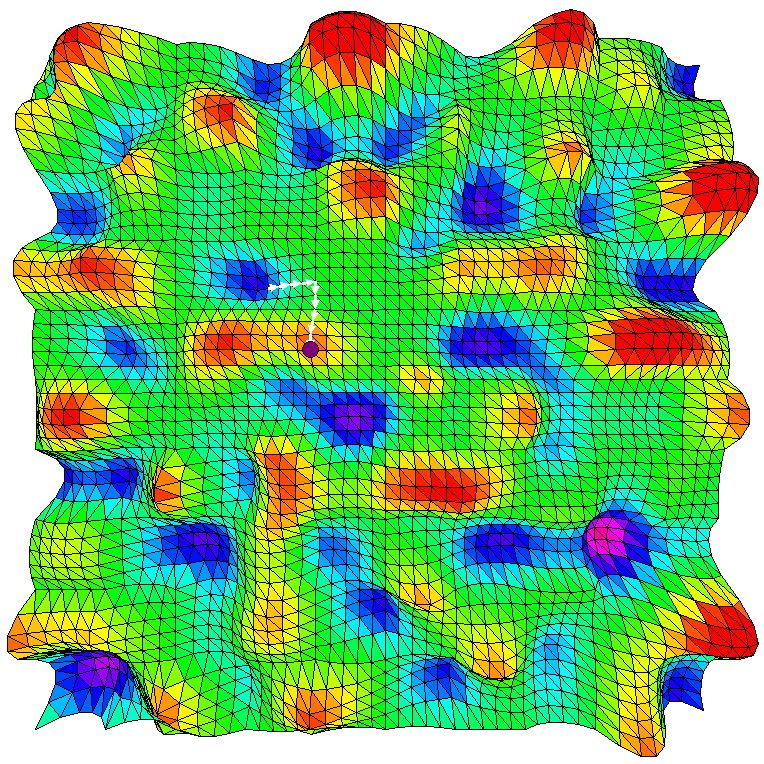
\includegraphics[width=\textwidth]{deep_q_learning/terrain_path_random_spawn.JPG}
        \caption{TODO}
        \label{img:pathDeepQRandomSpawn}
    \end{subfigure}
    \caption{Ergebnisse des ersten Experiments}
\end{figure}
Das Ergebnis lässt sich diesmal als Erfolg bezeichnen. Der Agent läuft von seiner Startposition so lange nach oben, bis es nicht mehr weiter nach oben geht. Einer dieser möglichen Pfade ist in Abbildung \ref{img:graphDeepQRandomSpawn} zu sehen. Die Aufgabe ist allerdings zu einfach. Im Graph \ref{img:graphDeepQRandomSpawn} lässt sich erkennen, dass der Großteil des Lernvorgangs bereits vor der 100-Epsioden-Marke passiert. Dies ist nicht optimal für unsere Zwecke, da wir erst ab Episode 100 den moving average und damit unsere Hauptvergleichsquelle verfolgen können.

Das neue Ziel ist daher, dass der Agent nicht nur nach oben läuft, sondern einen möglichst hohen Punkt in der Nähe des Startpunktes findet. Zu diesem Zweck erweitern wir die Eingaben, die das DQN bekommt. Wir übergeben nun die Höhe und die relative Position des in diesem Zeitschritt bisher höchsten besuchten Feldes. Außerdem wird die Anzahl der übrigen und der maximalen Zeitschritte angefügt. Dies soll in der Theorie dazu führen, dass der Agent seine Umgebung erkundet, solange noch genügend Zeit ist. Gegen Ende der Episode sollte er dann zum bisher höchsten bekannten Gipfel laufen.
\begin{figure}[H]
    \centering
    \begin{subfigure}[b]{0.49\textwidth}
        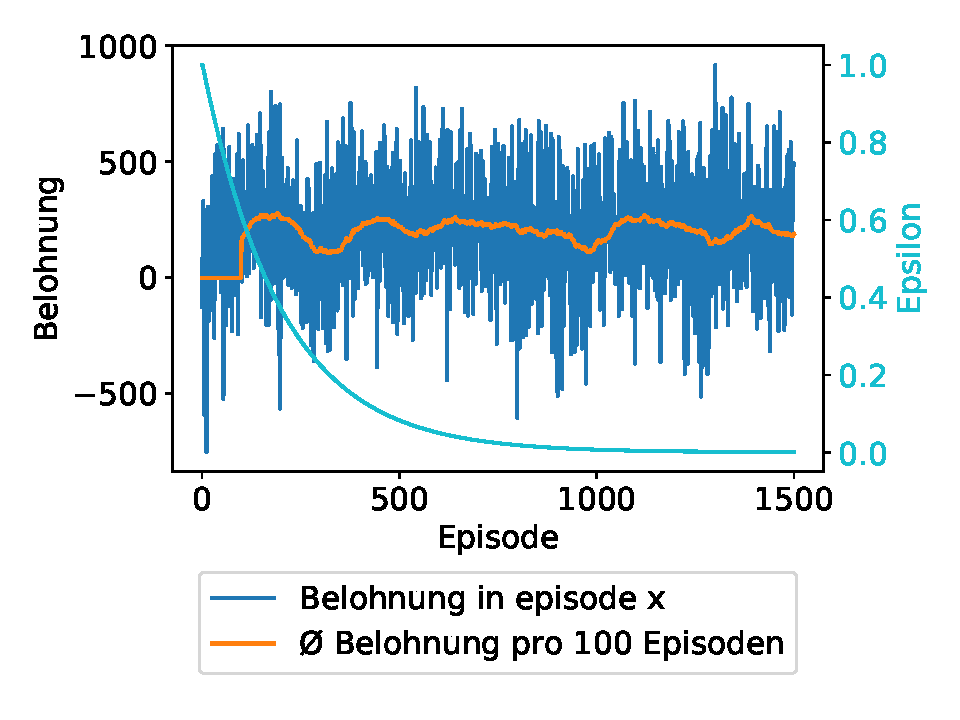
\includegraphics[width=\textwidth]{deep_q_learning/figure_random_spawn_2.pdf}
        \caption{TODO}
        \label{img:graphDeepQRandomSpawn2}
    \end{subfigure}
    \begin{subfigure}[b]{0.49\textwidth}
        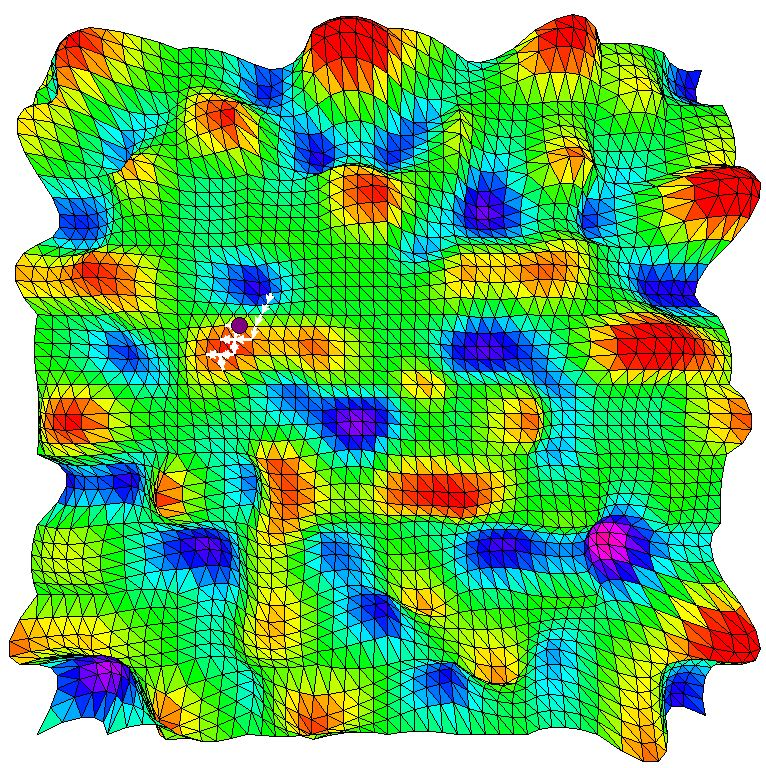
\includegraphics[width=\textwidth]{deep_q_learning/terrain_path_random_spawn_2.JPG}
        \caption{TODO}
        \label{img:pathDeepQRandomSpawn2}
    \end{subfigure}
    \caption{Ergebnisse des ersten Experiments}
\end{figure}
Das Ergebnis ist ähnlich wie das des vorangegangenen Experiments. Zum besseren Vergleich haben wir für die Darstellung in Abbildung \ref{img:pathDeepQRandomSpawn2} denselben Startpunkt gewählt wie in Abbildung \ref{img:pathDeepQRandomSpawn}. Der Agent orientiert sich tatsächlich hin zum etwas höheren Gipfel und scheint in einem sehr kleinen Umkreis die Umgebung zu erkunden, versäumt es aber am Ende auf dem höchsten Punkt aufzuhören. Dies kann  daran liegen, dass sich der Agent in jedem Zeitschritt bewegen muss und auf diese Weise nicht die Möglichkeit besitzt, genau auf dem höchsten Feld aufzuhören. Die Farbcodierung der Landschaft verrät uns allerdings, dass das Feld links oder unterhalb des vorletzten Schritts höher gelegen ist als das gewählte obere Feld. Viel wichtiger ist jedoch, dass der Graph \ref{img:graphDeepQRandomSpawn2} keinen wirklichen Trainingsfortschritt zeigt. Der moving average pendelt hier grob um denselben Wert und zeigt keinerlei Verbesserung des Agenten über längere Zeit. Auch dieser Ansatz ist also für unsere Zwecke nicht geeignet.

\paragraph{TODO}
Aufgrund der Misserfolge mit dem Finden von hohen Gipfeln wollen wir nun versuchen, ein anderes Ziel zu erarbeiten. Die neue Idee ist, dass der Agent so viele Felder wie möglich besuchen soll, sich dabei aber so wenig wie möglich vom Startfeld entfernt. Wir erhoffen uns hiervon, dass die quasi gegensätzlichen Ziele zu interessanten Ergebnissen führen und für ein DQN ein angemessenes Problem darstellen.

Um dieses Verhalten zu erreichen, werden sowohl die Beschreibung eines Zustands als auch die Belohnung stark angepasst. Die Belohnung setzt sich aus den beiden Aufgaben zusammen und sieht in etwa so aus:
\begin{minted}{python}
reward = (NEW_POINT_REWARD if is_new_point else 0) -\
         (DISTANCE_MULTIPLIER * distance_from_spawn)
\end{minted}
Der erste Part gibt den fixen Belohnungswert \mintinline{python}{NEW_POINT_REWARD} aus, falls das Feld vom Agenten noch nicht besucht wurde, ansonsten null. Davon wird dann die Distanz vom Startzustand abgezogen. Auf diese Weise erhält der Agent höhere Strafen je weiter er sich von diesem entfernt. Die Distanz wird davor noch mit einem ebenfalls fixen Wert \mintinline{python}{DISTANCE_MULTIPLIER} multipliziert. Die beiden fixen Werte (im Folgenden \textit{Belohnungsparameter} genannt) sollen als Stellschrauben dienen, um die richtige Gewichtung der beiden Ziele zu finden.

Als nächstes passen wir die Werte an, die einen Zustand beschreiben. Nicht mehr benötigt werden die Daten über die Höhe des eigenen und der umliegenden Felder. Stattdessen wird für jede angrenzende Position ein positiver Wert geliefert, wenn der Agent diese noch nicht besucht hat. Hat er das Feld schon besucht, so entspricht dieser Wert 0. Befindet sich der Agent am Rand der Landschaft und eines der angrenzenden Felder somit außerhalb des Grids, so wird der entsprechende Wert mit einer negativen Zahl belegt. Die Höhe der positiven und der negativen Wert lässt sich ebenfalls über einen fixen Parameter festlegen.
\begin{figure}[H]
    \centering
    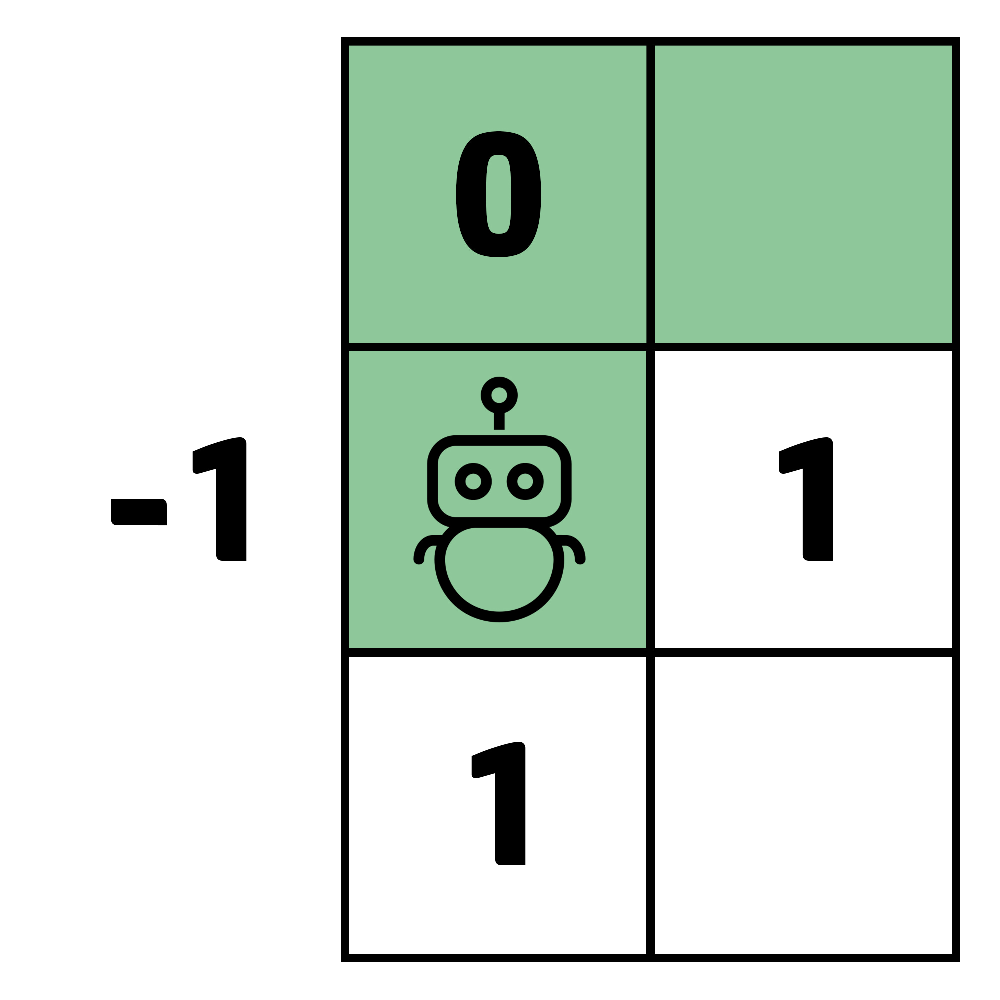
\includegraphics[width=0.3\textwidth]{state_visualisation.pdf}
    \caption{TODO} \label{img:stateVisualisation}
\end{figure}
Abbildung \ref{img:stateVisualisation} zeigt, wie die entsprechenden Werte ohne Multiplikator aussehen würden. Das Raster stellt einen kleinen Ausschnitt des Landschaft-Grids dar. Die grünen Felder hat der Agent bereits besucht. Das DQN erhält für das obere, bereits gesehene Feld also den Wert 0. Die beiden unerforschten Positionen rechts und unten liefern jeweils einen positiven Wert - in diesem Fall ohne einen Multiplikator also den Wert 1. Da die Position links des Agenten außerhalb des Grids liegt, ist diese mit dem Wert -1 belegt.

Die Werte bezüglich den Zeitschritten aus dem vorherigen Experiment sind ebenfalls enthalten. Insgesamt besteht ein Zustand jetzt also aus 8 Werten: Die relative Position (2), die Information über die anliegenden Positionen (4) und die Werte der übrigen beziehungsweise maximalen Zeitschritte (2).
\begin{figure}[H]
    \centering
    \begin{subfigure}[b]{0.59\textwidth}
        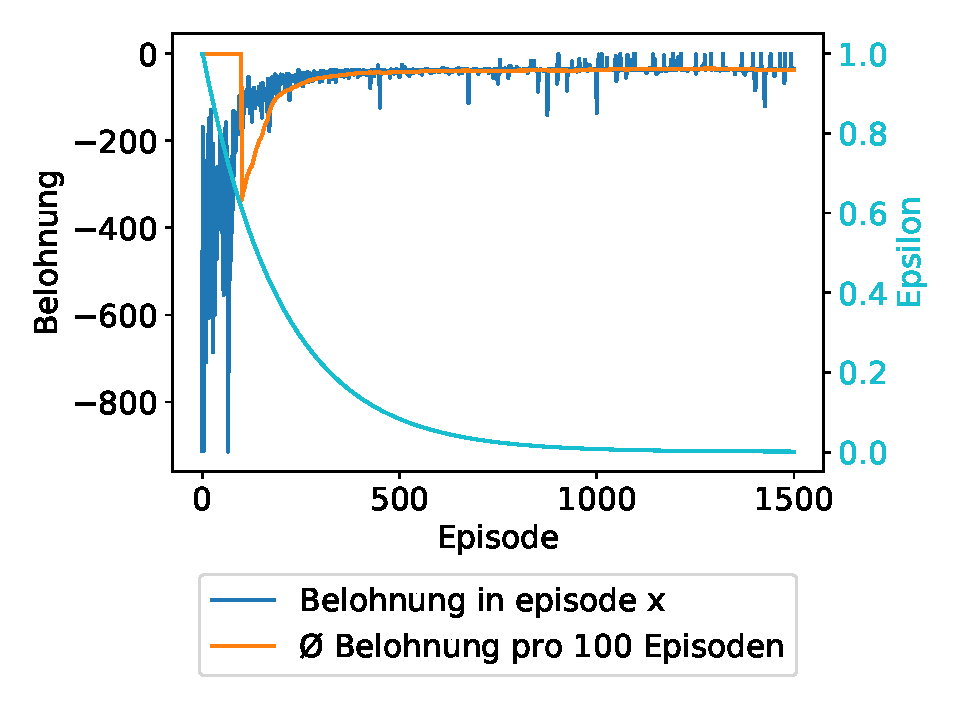
\includegraphics[width=\textwidth]{deep_q_learning/figure_random_spawn_spiral_1.pdf}
        \caption{TODO}
        \label{img:graphDeepQRandomSpawnSpiral1}
    \end{subfigure}
    \begin{subfigure}[b]{0.4\textwidth}
        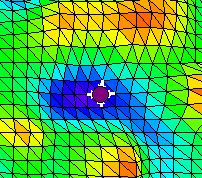
\includegraphics[width=\textwidth]{deep_q_learning/terrain_path_random_spawn_spiral_1_detail.JPG}
        \caption{TODO}
        \label{img:pathDeepQRandomSpawnSpiral1}
    \end{subfigure}
    \caption{Ergebnisse des ersten Experiments}
\end{figure}
Der Graph \ref{img:graphDeepQRandomSpawnSpiral1} zeigt wieder die Trainingsergebnisse der 1500 Episoden an. Am moving average lässt sich diemal ein sauberer Lernfortschritt erkennen. Die durchschnittliche Belohnung steigt bis circa Episode 400 stark an und flacht dann langsam ab. Dieser Verlauf ist sehr zufriedenstellend. Weniger zufriedenstellend ist allerdings das Verhalten, welches der Agent unter Verwendung des erlernten DQNs zeigt. Wie in Abbildung \ref{img:pathDeepQRandomSpawnSpiral1} zu sehen ist, bewegt sich der Agent von seiner Startposition aus lediglich ein Feld in jede Richtung und springt dann nur noch hin und her.
An dieser Stelle kommen unsere Belohnungsparameter zur Geltung. Da es dem Agenten aktuell wichtiger zu sein scheint, sich so wenig wie möglich vom Startpunkt zu entfernen, setzen wir den \mintinline{python}{NEW_POINT_REWARD} auf 10.
\begin{figure}[H]
    \centering
    \begin{subfigure}[b]{0.59\textwidth}
        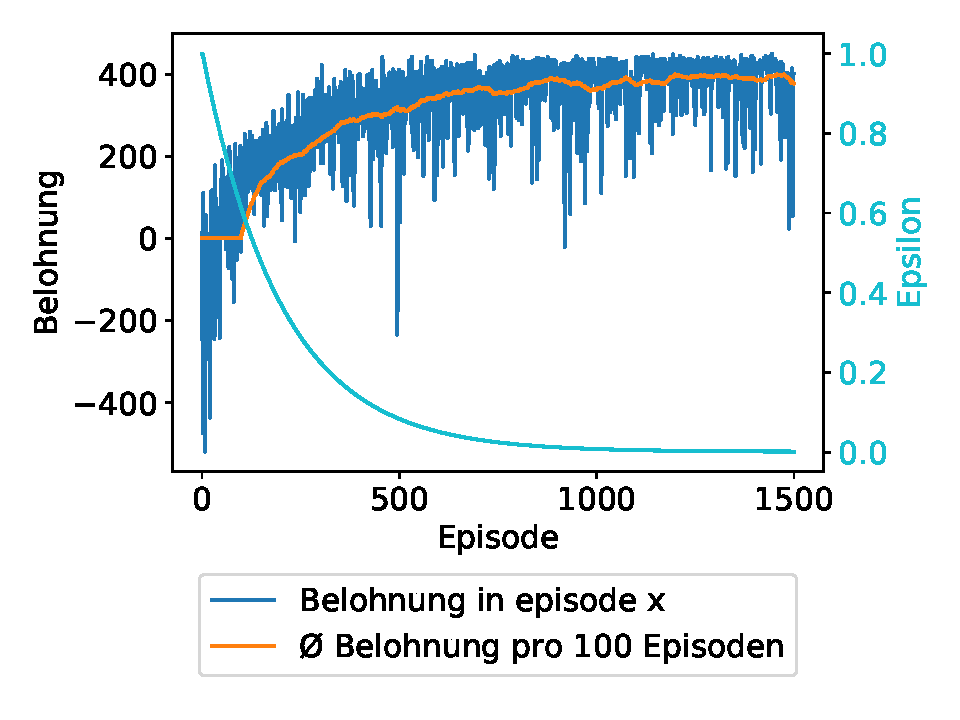
\includegraphics[width=\textwidth]{deep_q_learning/figure_random_spawn_spiral_2.pdf}
        \caption{TODO}
        \label{img:graphDeepQRandomSpawnSpiral2}
    \end{subfigure}
    \begin{subfigure}[b]{0.4\textwidth}
        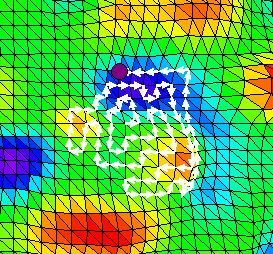
\includegraphics[width=\textwidth]{deep_q_learning/terrain_path_random_spawn_spiral_2_detail.JPG}
        \caption{TODO}
        \label{img:pathDeepQRandomSpawnSpiral2}
    \end{subfigure}
    \caption{Ergebnisse des ersten Experiments}
\end{figure}
Dies hat einen sehr positiven Einfluss auf das Ergebnis. Abbildung \ref{img:pathDeepQRandomSpawnSpiral2} stellt einen Pfad des Agenten nach dem Training dar. Die Startposition liegt hier etwa in der Mitte der abgelaufenen Fläche und der Agent läuft quasi spiralförmig immer weiter von diesem Punkt weg. Für das Lösen der Aufgabe ist das eine sehr gute Strategie, da viele neue Felder besucht werden und die Distanz zum Startpunkt gleichzeitig so gering wie möglich gehalten wird.

Der Graph \ref{img:graphDeepQRandomSpawnSpiral2} zeigt wie im Experiment davor eine schöne Lernkurve, welche zu Beginn des Trainings stark ansteigt und dann langsam abflacht. Aufgrund der höheren Belohnung für neu besuchte Felder verläuft der moving average nun im positiven Bereich.

\paragraph{}
Aufgrund dieser positiven Resultate mit dem Experiment werden wir diese Aufgabe für die Durchführung der weiteren Experimente nutzen und die Performance der unterschiedlichen Strategien vergleichen.
% Besser sind 2000 Episoden -> Test mit 10 Iterationen aus den Versuchen extrahieren

% test mit standart reward -> Zu einfach
% Stärke von DQN ausnutzen
% Zufälliger Spawn -> relative pos, sonst gleich -> läuft auf nächsten Berg
% Idee: Finde höchsten Berg in unmittelbarer Nähe, TODO State -> läuft trotzdem nur nach oben
% Neue Aufgabe: Decke so viel Fläche wie möglich ab, aber bleibe dabei so Nahe wie möglich am Spawn (eine Art Spirale)
% -> Gut, um Ergebnisse zu vergleichen
% 

\subsection{Experimente mit unterschiedlichen Strategien}
Im Graph \ref{img:graphDeepQRandomSpawnSpiral2} erkennt man, dass sich der moving average gegen Ende kaum noch verändert. Er steigt allerdings bis kurz davor noch minimal an, weswegen wir die Episodenlänge -- also die Zeitschritte pro Episode -- auf 2000 erhöhen. So soll sich auch bei langsameren Lernkurven der moving average am Ende bei einem Wert eingependelt haben. Es ist außerdem wichtig zu erwähnen, dass für die zufällige Wahl der Startposition für alle Experimentreihen der gleiche Seed benutzt wird. Die zufälligen Spawnpunkte und deren Reihenfolge sind also für alle Experimente gleich und somit besitzen alle die gleichen Voraussetzungen.

\paragraph{Experimentreihe mit den erarbeiteten Parametern}
Wir führen zunächst eine Experimentreihe mit den in Kapitel \ref{sec:deepQFirstExperiments} erarbeiteten Parametern (bis auf die\linebreak\mintinline{python}{max_steps_per_episode}) durch. Das Experiment wird wie in \ref{sec:qLearningExperiments} 20 Mal wiederholt. Bei den folgenden Graphen handelt es sich -- falls nicht anders angegeben -- immer um den durchschnittlichen moving average Wert und dessen Standardabweichung, welche als leicht transparenten Bereich um die Linie dargestellt wird.
\begin{figure}[H]
    \centering
    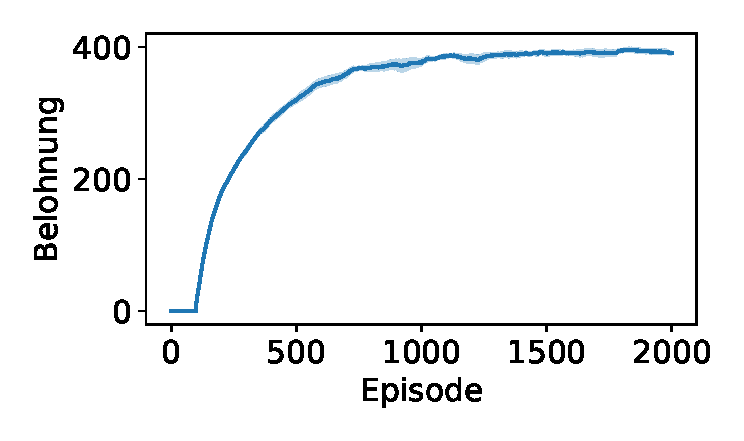
\includegraphics[width=0.5\textwidth]{deep_q_learning/figure_mean_dec_eps_1.pdf}
    \caption{TODO} \label{img:graphDeepQMeanDecEps1}
\end{figure}
Der Lernfortschritt scheint auch über mehrere Experimente hinweg sehr konsistent zu sein. Die Lernkurve verläuft im Graph \ref{img:graphDeepQMeanDecEps1} wie gewünscht anfangs steil und flacht gegen Ende ab. Die Standardabweichung ist zu jedem Zeitpunkt sehr gering, die Ergebnisse der Einzelexperimente unterscheiden sich also nicht stark voneinander. 

\paragraph{Agent ohne Erkundungsstrategie}
Anders verhält es sich beim Training ohne Erkundungsstrategie. Wir setzen hierfür unser $ \epsilon $ konstant auf 0. Der Agent agiert also wieder nur greedy. Auch dieses Experiment wiederholen wir 20 Mal.
\begin{figure}[H]
    \centering
    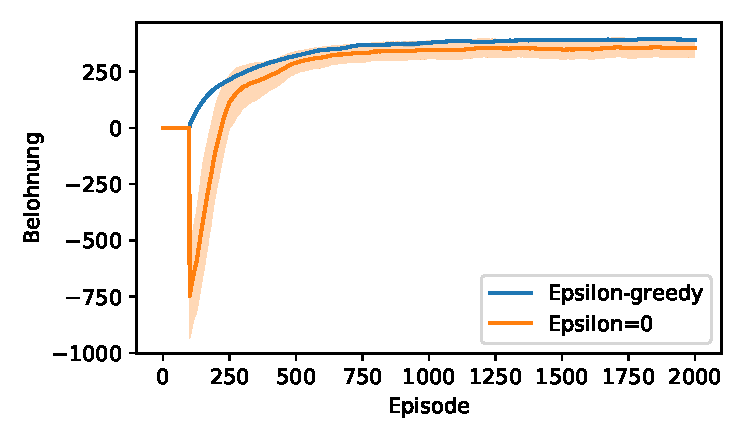
\includegraphics[width=0.8\textwidth]{deep_q_learning/figure_mean_stat_eps_0_vs_dec_eps_1.pdf}
    \caption{TODO} \label{img:graphDeepQMeanStatEps0VsDecEps1}
\end{figure}
Graph \ref{img:graphDeepQMeanStatEps0VsDecEps1} zeigt das Resultat dieses Experiments (orange Linie) und nochmals zum Vergleich das Resultat aus \ref{img:graphDeepQMeanDecEps1} (blaue Linie). Es fällt auf, dass die orange Linie wesentlich weiter unten beginnt als die blaue. Das bedeutet, dass der Agent ohne die $ \epsilon $-greedy Strategie langsamer lernt. Außerdem erreicht dieser nicht das gleiche Belohnungsmaximum. Dazu kommt, dass die Standardabweichung sichtbar größer ist. Der Lernerfolg ist demnach zusätzlich weniger zuverlässig. So zeigt sich erneut, dass eine Erkundungsstrategie die Performance des Agenten deutlich verbessert.

\paragraph{Konstante $ \epsilon $-Werte}
Als zusätzlichen Vergleich führen wir zwei weitere Experimente mit konstantem $ \epsilon $ durch. Wir setzen hierfür $ \epsilon = 0.2 $ und $ \epsilon = 0.5 $.
\begin{figure}[H]
    \centering
    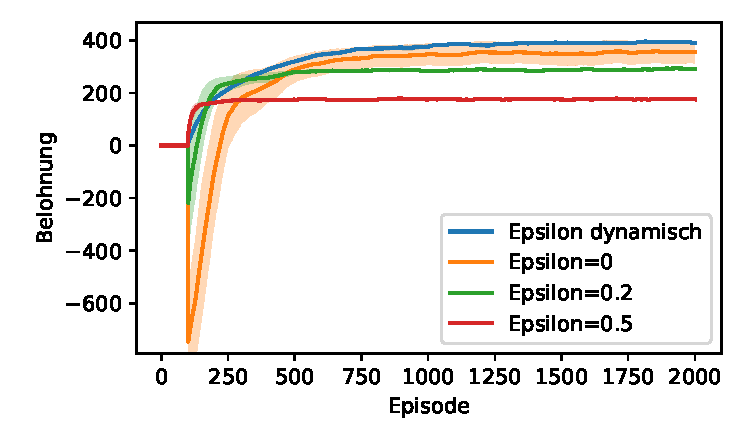
\includegraphics[width=0.8\textwidth]{deep_q_learning/figure_mean_eps_comparison.pdf}
    \caption{TODO} \label{img:graphEpsComparison}
\end{figure}
Auf den ersten Blick scheint ein Agent ohne Erkundungsstrategie (orange Linie) bessere Ergebnisse zu erzielen als die Agenten mit konstanten $ \epsilon $-Werten (grüne und rote Linie). Man darf hierbei allerdings nicht vergessen, dass diese ihr $ \epsilon $ nicht \glqq loswerden \grqq{}, sondern bis zum Ende immer mit der Wahrscheinichkeit $ \epsilon $ eine zufällige Aktion wählen. Da das willkürliche Vorgehen natürlich keine gute Strategie ist, ist im Graphen \ref{img:graphEpsComparison} auch der moving average der Experimente mit größerem, konstanten $ \epsilon $ geringer. Die tatsächliche Performance des Agenten wird quasi von dem fixen $ \epsilon $ sabotiert. Wir führen daher eine weitere Form der Datendarstellung ein: sogenannte Boxplots.
\begin{figure}[h!]
    \centering
    \begin{subfigure}[b]{0.7\textwidth}
        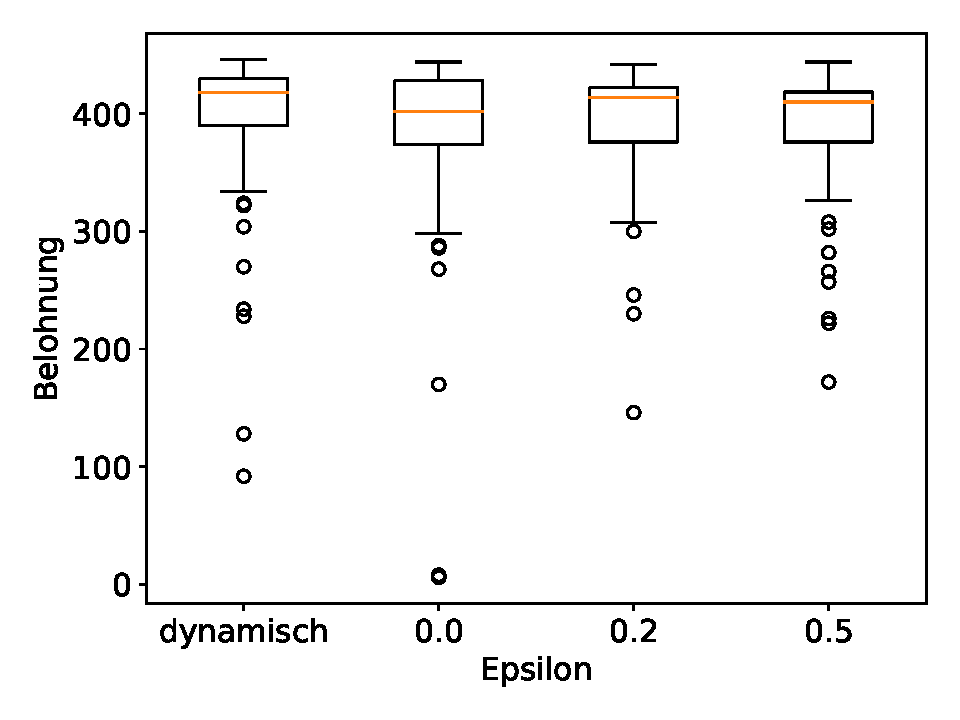
\includegraphics[width=\textwidth]{deep_q_learning/figure_box_eps_comparison.pdf}
        \caption{TODO}
        \label{img:graphBoxEpsComparison}
    \end{subfigure}
    \begin{subfigure}[b]{0.7\textwidth}
        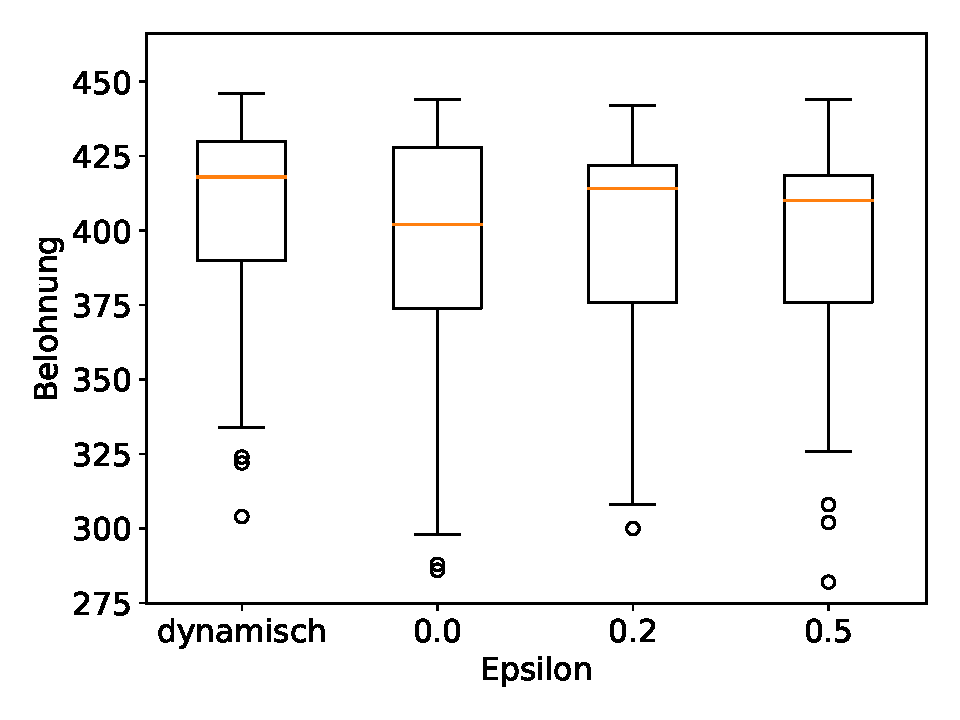
\includegraphics[width=\textwidth]{deep_q_learning/figure_box_eps_comparison_big.pdf}
        \caption{TODO}
        \label{img:graphBoxEpsComparisonBig}
    \end{subfigure}
    \caption{Ergebnisse des ersten Experiments}
\end{figure} \label{img:graphBoxEpsComparisonBoth}

(TODO Boxplots an sich erklären?) Die Boxplots sollen das Verhalten des Agenten unter Anwendung des erlernten DQNs beschreiben. Die y-Achse in den Plots \ref{img:graphBoxEpsComparisonBoth} zeigt wieder die Summe der Belohnungen innerhalb einer Episode an. Die x-Achse beschreibt, um welches Experiment es sich handelt, also in diesem Fall welches $ \epsilon $ benutzt wurde. Von links nach rechts sind das in diesem Fall unser dynamisches $ \epsilon $ gefolgt von den drei fixen Werten 0.0, 0.2 und 0.5. Jedes Experiment wurde bisher 20 Mal durchgeführt. Das bedeutet, dass wir für jede Experimentenreihe 20 trainierte DQNs besitzen. Der Agent durchläuft nun mehrere Iterationen, wobei er jedes dieser Netze 5 Mal in der Umgebung anwendet. Pro Experimentreihe erhalten wir also 100 Belohnungssummen, welche wir in einem Boxplot darstellen. Der Seed für die Startposition wird zu Beginn jedes Experiments zurückgesetzt, um gleiche Voraussetzungen zu gewährleisten. Der Graph \ref{img:graphBoxEpsComparison} zeigt die resultierenden Boxplots mit ihren Ausreißern. In \ref{img:graphBoxEpsComparisonBig} wurden diese für die bessere Interpretation der Boxplots abgeschnitten.

Es lässt sich zunächst feststellen, dass der Median beim Boxplot des dynamischen $ \epsilon $ den höchsten Wert hat. Ebenso liegen aber auch die anderen Werte, also das 1. Quartil, das 3. Quartil, das Minimum und das Maximum, bei diesem Experiment am höchsten. Es lässt sich also klar sagen, dass ein über Zeit schrumpfendes Epsilon -- also die klassische $ \epsilon $-greedy Strategie -- in der Anwendung bei uns die beste Performance liefert.

Bei den Experimenten mit fixem Epsilon fällt als Erstes auf, dass das Minimum mit steigendem Epsilon immer größer wird. Wir interpretierend dies so, dass die Agenten mit einem größeren Epsilon mehr von ihrer Umgebung erkundet haben und daher für mehr Anwendungsfälle eine bessere Strategie habe. Dass der Median beim Epsilon von 0.5 wieder leicht niedriger ist als bei 0.2 kann eventuell bedeuten, dass ein zu großes Epsilon dazu führt, dass die bereits erkundeten Pfade weniger stark perfektioniert werden. Die Änderung ist allerdings relativ gering. Um hier eine eindeutige Aussage zu treffen bräuchten wir mehr Daten.

Wir haben allerdings einmal mehr gezeigt, dass sich die Erkundungsstrategie auf das Verhalten des Agenten auswirkt.

\subsection{Experimente mit Erkundungsstrategie über die Modifikation der Belohnung}
Im Folgenden soll die Erkundungsstrategie nur über die Belohnungs-Funktion implementiert werden. Wir modifizieren unseren Agenten also zunächst dahingehend, dass er in jedem Fall greedy agiert. Die Hyperparameter für Epsilon haben also keinen direkten Einfluss mehr auf die Wahl der Aktion.
\begin{minted}{python}
params = DeepQParameters(
            num_episodes=2000,
            max_steps_per_episode=80,
            replay_buffer_size=20000,
            batch_size=32,
            learning_rate=0.001,
            discount_rate=0.999,
            target_update=25,
            start_exploration_rate=1,
            max_exploration_rate=1,
            min_exploration_rate=0.001,
            exploration_decay_rate=0.005,
            # ... Rest wird erst während des Trainings belegt
        )
\end{minted}

\paragraph{TODO}
In Graph \ref{img:graphEpsComparison} lässt sich erkennen, dass die Belohnungssumme in einer Episode maximal circa 400 beträgt. Da eine Episode 80 Zeitschritte enthält, bekommt der Agent pro Zeitschritt eine durchschnittliche Belohnung von ungefähr 5. Wir nutzen dieses Wissen, um eine neue Belohnungs-Funktion zu formulieren:
\begin{minted}{python}
modified_reward = (1 - exploration_rate) * reward - exploration_rate * 5
\end{minted}
Ähnlich wie beim Q-Learning-Experiment soll der Agent so zu Beginn negative Belohnungen erhalten, damit er andere Pfade erkundet. Wir lassen den Agenten mit dieser Strategie ebenfalls 20 Mal trainieren. Da bei dieser Belohnugs-Funktion mit den aktuellen Hyperparametern am Anfang nichts von der tatsächlichen Belohnung übrig bleibt und der Agent auf diese Weise eventuell in den ersten Zeitschritten nichts lernt, führen wir noch ein weiteres Experiment durch, dessen Hyperparameter mit \mintinline{python}{start_exploration_rate=0.5} und \mintinline{python}{max_exploration_rate=0.5} belegt werden.

\begin{figure}[h!]
    \centering
    \begin{subfigure}[b]{0.49\textwidth}
        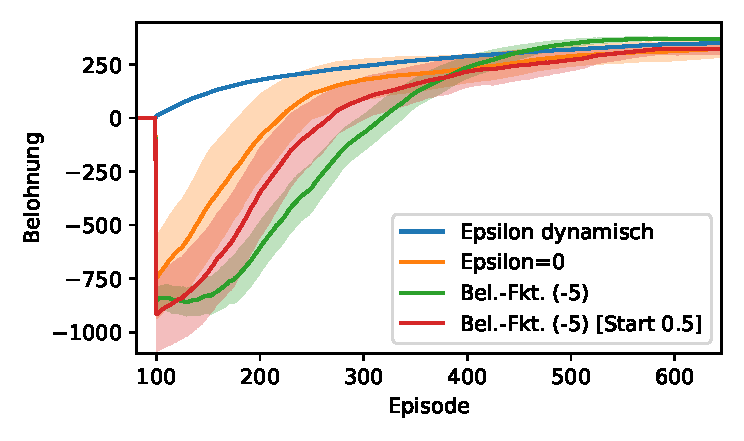
\includegraphics[width=\textwidth]{deep_q_learning/figure_mean_eps_5_in_rew_big.pdf}
        \caption{TODO}
        \label{img:graphEps5InRewBig}
    \end{subfigure}
    \begin{subfigure}[b]{0.49\textwidth}
        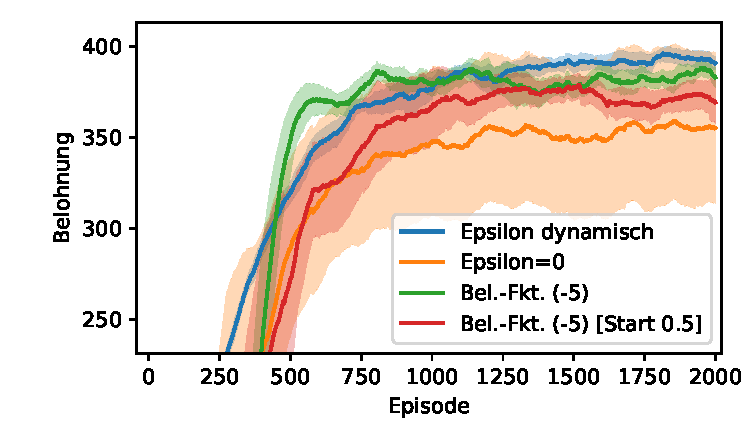
\includegraphics[width=\textwidth]{deep_q_learning/figure_mean_eps_5_in_rew_big2.pdf}
        \caption{TODO}
        \label{img:graphEps5InRewBig2}
    \end{subfigure}
    \begin{subfigure}[b]{0.7\textwidth}
        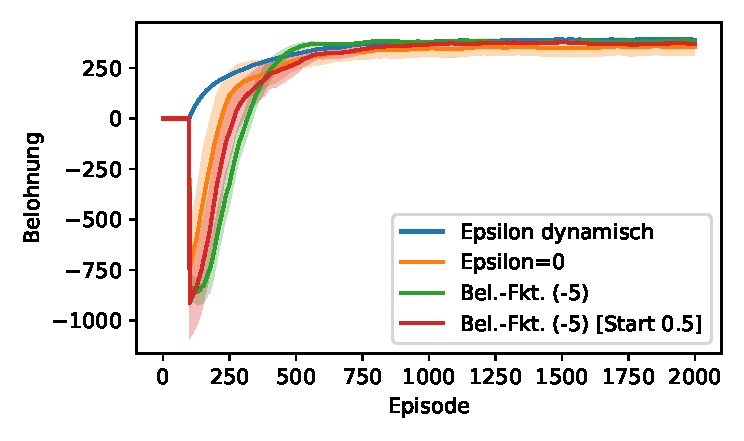
\includegraphics[width=\textwidth]{deep_q_learning/figure_mean_eps_5_in_rew.pdf}
        \caption{TODO}
        \label{img:graphEps5InRew}
    \end{subfigure}
    \caption{Ergebnisse des ersten Experiments}
\end{figure} \label{img:graphEps5InRewBoth}

Die Graphen in Abbildung \ref{img:graphEps5InRewBoth} zeigen wieder den durchschnittlichen moving average und dessen Standardabweichung für alle Episoden. Zum Vergleich sind hier noch die Werte für das klassische Epsilon (blau) und dem fixen Epsilon 0.0 (orange) eingetragen. Der Graph \ref{img:graphEps5InRew} enthält aller Werte. Der Graph \ref{img:graphEps5InRewBig} zeigt für einen detaillierten Vergleich des ersten Trainingsviertels die ersten 600 Episoden. Um die Unterschiede nach dem ersten Trainingsviertel besser erkennen zu können, zeigt der Graph \ref{img:graphEps5InRewBig2} einen Ausschnitt der Belohnungswerte von 250 bis 400.

Die grüne und die rote Linie zeigt den Trainingsverlauf unter Anwendung oder oben beschriebenen, modifizierten Belohnungs-Funktion, wobei letztere das Experiment mit \mintinline{python}{start_exploration_rate=0.5} und \mintinline{python}{max_exploration_rate=0.5} beschreibt. Beide liefern im ersten Viertel des Trainings schlechtere Belohnungswerte als das Training ohne Erkundungsstrategie. Danach überholen sie dieses allerdings und liegen am Ende zwischen dem Training mit Epsilon=0 und der klassischen $ \epsilon $-greedy Strategie. Zudem scheinen die Ergebnisse zuverlässiger zu sein als bei Epsilon=0, wie man von der wesentlich geringeren Standardabweichung ableiten kann.

Der Start mit einer geringeren \mintinline{python}{start_exploration_rate} führt wie erwartet am Anfang zu schnelleren Ergebnissen, wird allerdings von der Strategie, bei der die\linebreak\mintinline{python}{exploratrion_rate} bei 1 startet, überholt und scheint insgesamt etwas inkonsistentere Belohnungen zu liefern, was uns die Standardabweichung verrät.

Um zu beurteilen, wie sich der Agent nach dem Training verhält, sehen wir uns wieder die Boxplots an.

\begin{figure}[h!]
    \centering
    \begin{subfigure}[b]{0.7\textwidth}
        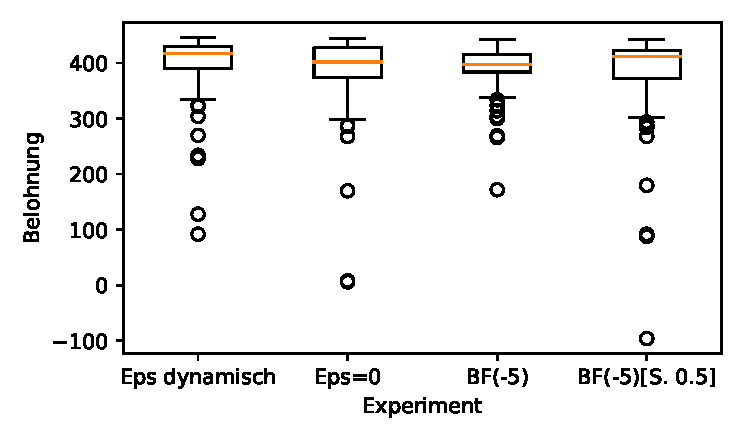
\includegraphics[width=\textwidth]{deep_q_learning/figure_box_eps_5_in_rew.pdf}
        \caption{TODO}
        \label{img:graphBoxEps5InRew}
    \end{subfigure}
    \begin{subfigure}[b]{0.7\textwidth}
        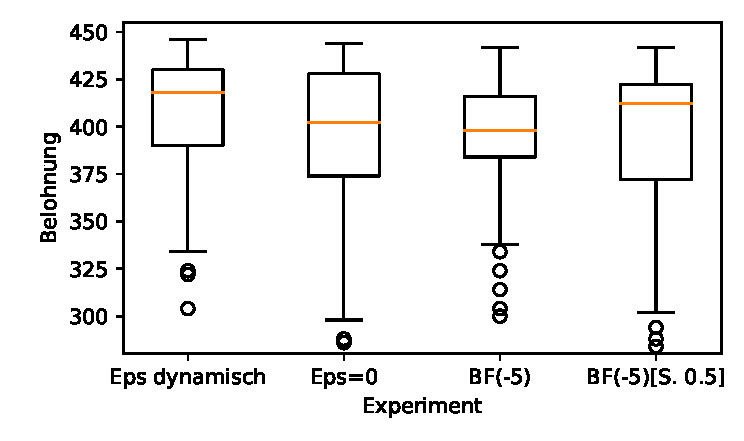
\includegraphics[width=\textwidth]{deep_q_learning/figure_box_eps_5_in_rew_big.pdf}
        \caption{TODO}
        \label{img:graphBoxEps5InRewBig}
    \end{subfigure}
    \caption{Ergebnisse des ersten Experiments}
\end{figure} \label{img:graphBoxEps5InRewBoth}

\paragraph{TODO}
Wir wollen nun versuchen, den Schwerpunkt noch etwas mehr auf die zufällige Erkundung der Umgebung zu setzen. Wir passen hierfür unsere Belohnungs-Funktion an:
\begin{minted}{python}
    modified_reward = (1 - exploration_rate) * reward -\
                      exploration_rate * random.uniform(0.0, 5.0)
\end{minted}
Die \mintinline{python}{exploration_rate} wird nun nicht mehr direkt mit unserem errechneten Wert 5 multipliziert, sondern mit einem zufälligen Wert zwischen 0 und 5. Dies soll die zufällige Wahl der Aktionen und damit die zufällige Erkundung der Umgebung gewissermaßen über die Belohnung abbilden.